\documentclass{if-beamer}
\usepackage[utf8]{inputenc}

% --------------------------------------------------- %
%                  Presentation info	              %
% --------------------------------------------------- %
\title[Adapter]{Design Patterns:}
\subtitle{Adapter}
\author{William Gabriel Pereira}
\institute[IFC]{
  Instituto Federal Catarinense\\
  Campus Rio do Sul
}
\date{\today}
\logo{

\includegraphics[scale=0.07]{Logo_vertical.png}
}
\subject{Presentation subject} % metadata

\graphicspath{{figuras/}}

% inicia o documento
\begin{document}

% insere slide titulo
\begin{frame}
	\titlepage
\end{frame}

% insere "sumario"
\begin{frame}{agenda}
	\tableofcontents
\end{frame}

% inicia nova sessão
\section{Design Patterns Estruturais}
\begin{frame}{Design Patterns Estruturais}
	% insere bloco	
	\begin{block}{O que é um padrão estrutural}
		Assim como os outros Design Patterns estudados anteriormente, estes padrões são usados para resolver problemas comuns entre os sistemas. A diferença é "o que" resolvem.	
	\end{block}
	\subsection{O que resolvem}
	\begin{block}{O que resolvem então?}
		Tratam a maneira de como as classes são armazenadas em um projeto, ou seja, esses padrões são envelopadores. É utilizada classe dentro de uma outra classe, modificando algo em tal  objeto/função, ainda em tempo de execução.
		Em suma, são classes que modificam a disposição e alteram funções de outras classes, tornando elas compativeis com o projeto.
	\end{block}
\end{frame}

\begin{frame}
	%\subsection{Quais são}
	\begin{block}{Padrões estruturais:}
	\begin{itemize}
		\item Adapter
		\item Bridge
		\item Composite
		\item Decorator
		\item Facade
		\item Flyweight
	\end{itemize}
	\end{block}

\end{frame}

\section{Adapter}
\begin{frame}{Adapter}
	\begin{block}{O que é}
		Como diz o deu próprio nome, o padrão Adapter é um padrão usado para adaptar uma classe, ou seja, serve para flexibilidade e compatibilidade.
	\end{block}

	\subsection{Como funciona}
	\begin{block}{Como funciona}
		Imagine o seguinte: você fez um sistema que utiliza uma {\itshape API} com {\itshape WEBSERVICE}, porém o {\itshape WEBSERVICE} foi fechado, então o que fazer? modificar todo o sistema para funcionar com uma nova {\itshape API}, certo? \emph{ERRADO}!
		\newline
		\newline
		Para não gastar muito tempo modificando todo o sistema, fazemos um adaptador, uma classe que acessa outra {\itshape WEBSERVICE}, porém sem mexer muito no código principal.
	\end{block}
\end{frame}

\begin{frame}

	\begin{block}{Outro exemplo}
		Vamos para um exemplo mais cotidiano. Quando temos uma tomada de pinos planos, porém a entrada da tomada é de pinos redondos, o que fazemos?

		Em casos extremos, trocamos a ponta da tomada, mas somente em casos realmente extremos. Geralmente corremos atrás de um {\itshape T}, ou um adaptador.

		\boxorange{	O Adapter é exatamente isso, o intermediário, o adaptador de tomada.}
	\end{block}

	\begin{figure}
		\centering
		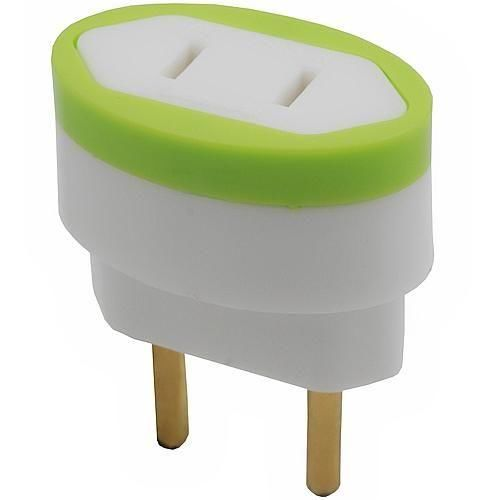
\includegraphics[scale=0.10]{adaptador.jpg}
	\end{figure}
\end{frame}

\section{Definição}
\begin{frame}{Definição Oficial}
	\definecolor{ofc}{rgb}{0.9,0.3,0}
	\begin{block}{}
		\textbf{\textcolor{ofc}{O Padrão Adapter converte uma interface de uma classe para outra interface que o cliente espera encontrar. O Adaptador permite que classes com interfaces incompatíveis trabalhem juntas}}
	\end{block}

	\begin{exampleblock}{}
		{\itshape "Se anda como um pato, grasna como um pato, então talvez seja peru envelopado num adaptador de pato"}
	\end{exampleblock}
\end{frame}

\section{Programando}
\begin{frame}{Programando}
	
	\begin{alertblock}{Interface}
		Para que funcione, precisamos de uma interface com as funções que são implementadas na classe que desejamos modificar, neste caso a {\itshape TomadaPlana}.

		O cliente vai estar solicitando a função pela interface, porém a implementação da interface vai estar no adaptador, que vai chamar a função equivalente da {\itshape TomadaCircular}.
	\end{alertblock}

	\begin{figure}
		\centering
		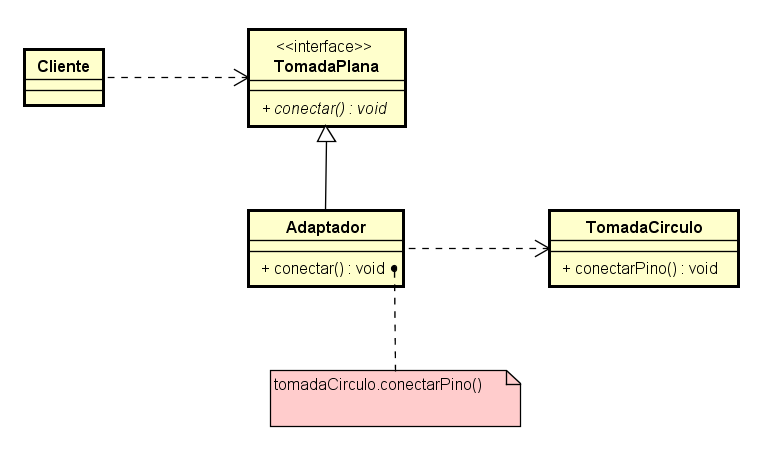
\includegraphics[scale=0.5]{diagrama.png}
		\caption{Diagrama do exemplo tomada}
	\end{figure}
\end{frame}

\begin{frame}
	
	\subsection{Interfaces}
	\begin{exampleblock}

		Implementar primeiro as interfaces:
		\begin{itemize}
			\item ITomadaPlana
			\item ITomadaCircular
		\end{itemize}
	\end{exampleblock}

	\lstinputlisting[language=Java, firstline=3] {../adapter/src/tomada/ITomadaPlana.java}
	
	\lstinputlisting[language=Java, firstline=3] {../adapter/src/tomada/ITomadaCircular.java}
\end{frame}

\begin{frame}

	\subsection{Classes concretas}	
	\begin{exampleblock}

		Implementar então as classes concretas:
		\begin{itemize}
			\item TomadaPlana
			\item TomadaCircular
		\end{itemize}
	\end{exampleblock}

	\lstinputlisting[language=Java, firstline=3] {../adapter/src/tomada/TomadaPlana.java}
	
	\lstinputlisting[language=Java, firstline=3] {../adapter/src/tomada/TomadaCircular.java}

\end{frame}

\begin{frame}
	
	\subsection{Factory}
	\begin{exampleblock}

		Usei uma Factory para encapsular melhor as classes não Main
	\end{exampleblock}

	\lstinputlisting[language=Java, firstline=3, lastline=6] {../adapter/src/tomada/Factory.java}

\end{frame}

\begin{frame}
	
	\subsection{Main}
	\begin{exampleblock}

		Façamos então uma classe Main para testar as classes que vamos adaptar antes de adaptar
	\end{exampleblock}

	\lstinputlisting[language=Java, firstline=3] {../adapter/src/tomada/Main.java}

	\boxyellow{Conectado Plano}

	\lstinputlisting[language=Java, firstline=3] {../adapter/src/tomada/Main2.java}

	\boxyellow{Conectado circulo}


\end{frame}

\begin{frame}
	
	\subsection{Adapter em si}
	\begin{exampleblock}

		Agora sim vamos implementar a classe adaptadora
	\end{exampleblock}

	\lstinputlisting[language=Java, firstline=3] {../adapter/src/tomada/Adaptador.java}

\end{frame}

\begin{frame}
	
	\begin{exampleblock}

		Agora façamos essa pequena alteração na classe Factory e rodemos o primeiro Main
	\end{exampleblock}

	\lstinputlisting[language=Java, firstline=8, lastline=10] {../adapter/src/tomada/Factory.java}

	\begin{alertblock}

		Em teoria, a tomada plana deveria conectar em tomada plana, porém com o adaptador temos como print o seguinte: \boxyellow{Conectado circulo}
	\end{alertblock}

\end{frame}

\section{Água em vinho}
\begin{frame}{Água em vinho}
	\begin{block}

		Podemos com isso, brincar de Jesus, vamos transformar a água em vinho agora!
	\end{block}
	\subsection{ICopoAgua}
	\subsection{Vinho}
	\begin{block}{ICopoAgua}
		\lstinputlisting[language=Java, firstline=3] {../adapter/src/jesus/ICopoAgua.java}
	\end{block}

	\begin{block}{Vinho}
		\lstinputlisting[language=Java, firstline=3] {../adapter/src/jesus/Vinho.java}
	\end{block}
\end{frame}

\begin{frame}

	\subsection{Jesus}
	\begin{block}{Jesus}
		\lstinputlisting[language=Java, firstline=3] {../adapter/src/jesus/Jesus.java}
	\end{block}

	\subsection{Factory}
	\begin{block}{Factory}
		\lstinputlisting[language=Java, firstline=3] {../adapter/src/jesus/Factory.java}
	\end{block}

	
\end{frame}

\begin{frame}

	\begin{block}{Main}
		\lstinputlisting[language=Java, firstline=3] {../adapter/src/jesus/Main.java}
	\end{block}

	\begin{exampleblock}

		Temos como resultado disso tudo a transformação da água em vinho ao rodar o nosso Main

		\boxyellow{Cheio de vinho!}
	\end{exampleblock}
\end{frame}

\end{document}
